
\chapter{Experimental analysis of existing solutions}

\label{seq:analysis}

In this chapter we provide an assessment of the the quality and stability of the 7pt algorithm (algorithm~\ref{7pt}) with the Bougnoux formula (Eq.~\ref{eq:bougnoux1}). We consider this pipeline as essentially integral baseline procedure for estimation of the focal lengths from image correspondences.


\section{Experimental setup}


We assume zero skew and unity aspect ratio in both cameras and consider a partially calibrated problem, i.e., the principal points are known. We assume that the images were preprocessed in a way that principal points are always in the center. This means that the calibration matrices after this preprocessing are of shape \[ \mathtt{K}_i = \mat{ccc}{f_i & 0 & 0 \\ 0 & f_i & 0 \\ 0 & 0 & 1}. \] Different cameras are allowed to have different focal lengths.

\subsection{Evaluation procedure}
The setup for most experiments in the work is as follows:

\begin{algorithm}[H]
\SetAlgoNoLine
\LinesNumbered
 \KwData{The number of correspondences used $n$, noise $\sigma$}
 \Begin
    {Create a camera pair $\mathtt{P}_1$, $\mathtt{P}_2$ with focal lengths $f_1$,$f_2$\; 
 
    Create a point cloud $\mathtt{X} \in \mathbb{R}^{3 \times n}$ of $n$ points in 3D \;
    
    Project $\mathtt{X}$ to the cameras $\mathtt{P}_1$ and $\mathtt{P}_2$, producing the ground truth image point sets ${\mathtt{x}}_1^{gt}$, ${\mathtt{x}}_2^{gt} \in \mathbb{R}^{2 \times n}$ \;
    
    
    Apply additive noise drawn from $\mathcal{N}(0,\,\sigma^{2})$ to both $x$, $y$ coordinates of each point from ${\mathtt{x}}_1^{gt}$ and ${\mathtt{x}}_2^{gt}$. This produces observed image point sets $\mathtt{x}_1^{ob}$ and $\mathtt{x}_2^{ob}$ correspondingly \;
    
    Select 7 pairs of corresponding points $\mathtt{x}_1$ and $\mathtt{x}_2$, and let the remaining pairs to be the test set $\mathtt{x}_1^{test}, \mathtt{x}_2^{test}$ \;
    
    Get the $\mathtt{F}_i$ estimates of the fundamental matrix $\mathtt{F}$ from the correspondences $\mathtt{x}_1,\mathtt{x}_2$  (e.g. $i = 1\dots 3$ when using the 7pt algorithm (algorithm~\ref{7pt})). Leave only matrices with real elements\;
    
    %Choose the estimation that has the most support points from test set using the voting procedure\;
    Choose the estimation that optimizes Sampson error (equation~\ref{eq:sampson}) on the test set\;
    
    Estimate the focal lengths from the fundamental matrix $\mathtt{F}$ using the formulae~\ref{eq:bougnoux1} and \ref{eq:bougnoux2}\;
    }
 \caption{Workflow}
 \label{workflow}
\end{algorithm}

%The voting procedure allows to choose a fundamental matrix that fits data with big 

\subsection{Estimation quality measure}
\begin{figure}[h!]
      \begin{center}
    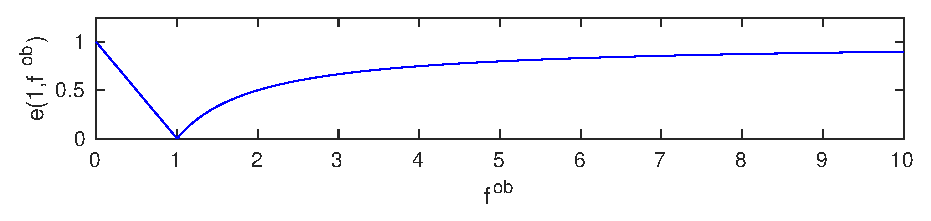
\includegraphics[width=\linewidth]{error_eval.eps}
    \caption[Focal length error function]{Error function \ref{eq:error} for the focal length, where $f_{gt}$ is fixed to 1.}
    \label{fig:error}
  \end{center}
\end{figure}
We treat error in focal length estimation as multiplicative, so that the error in case where the ground truth $f_{gt}=1000$ and computed value $f_{ob}=2000$ is the same as error in case where the ground truth $f_{gt}=100$ and computed value $f_{ob}=200$. More precisely the error is given by 
\begin{equation}
e(f_{gt},f_{ob})= 1 - \frac{\min(f_{gt}, f_{ob})}{\max(f_{gt}, f_{ob})}.
\label{eq:error}
\end{equation} The error function for fixed ground truth value $f_{gt}=1$ is shown in the Fig.~\ref{fig:error}.  

For measuring the quality of a fundamental matrix we use the Sampson error: 
\begin{equation}
S(\mathtt{F}) = \sum_i \frac{(\mathbf{x}_2^\T \mathtt{F} \mathbf{x}_1)^2}{(\mathtt{F} \mathbf{x}_1)_1^2 + (\mathtt{F} \mathbf{x}_1)_2^2 + (\mathbf{x}_2^\T \mathtt{F})_1^2 + (\mathbf{x}_2^\T \mathtt{F})_2^2}.
\label{eq:sampson}
\end{equation}


\section{Performance analysis for generic situations}

In this section we analyze the focal length computation performance for a generic scene, in which a degeneracy is unlikely to occur. 

In experiments, we each time generate a random set of points and a random camera pair so that the set of correspondences in each image span at least 1000 $\times$ 1000 pixel square. 


\subsection{Overall analysis}
We analyze the behavior of the pipeline against different numbers of given correspondences and different levels of noise. The quality of the estimation is assessed by computing the median of focal lengths computation  error $e$ and its 0.25 and 0.75 quantiles. In these experiments we discard each all imaginary estimates.

The Fig.~\ref{mean_v_corrs} shows a rapid decline in error with growing number of correspondences. This is explained by the fact that both algorithms use SVD procedure to optimize error on epipolar constraints. With bigger number of correspondences the error caused by random noise is averaged and the estimation becomes more stable. %Using 20 correspondences we can achieve an error close to negligible.
% This may be explained by the known fact that the 8pt solver optimizes error of matrix $\mathtt{F}$ in a certain sense \TP{Explain better. What do you mean by "certain sense"? What do you mean by "error of matrix"?}, as described by ? in~\cite{}. 

\begin{figure}[h!]
  \begin{center}
    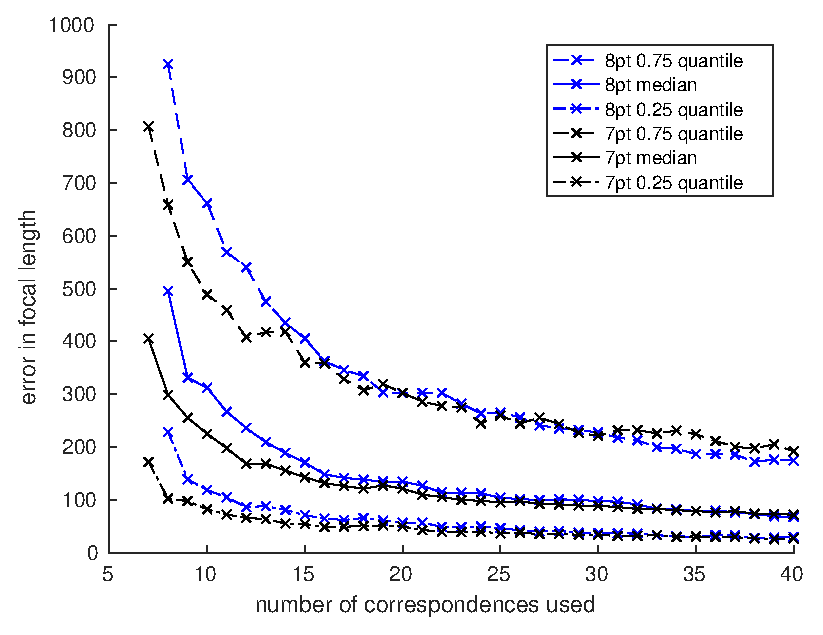
\includegraphics[width=\linewidth]{mean_error_corrs.eps}
    \caption[Error in focal length versus number of correspondences]{A Comparison of the 7pt and 8pt algorithms against the number of correspondences used. Median error $f - f^{true}$ in focal length and two its 0.25, 0.75 quantiles are shown. The ground truth $f^{true}$ is equal to 1500. The level of noise $\sigma$ is equal to 1. Imaginary estimates are excluded. }
    \label{mean_v_corrs}
  \end{center}
\end{figure}

The Fig.~\ref{mean_v_noise} shows the growth of the error with increasing noise. The number of  correspondences used is 8 for both algorithms. We see that the error growth is approximately linear and quite mild, e.g., with additive noise of 3 pixels the error is still bearable. For realistic values of noise around 1 pixel, the error is reasonably small.



\begin{figure}[h!]
  \begin{center}
    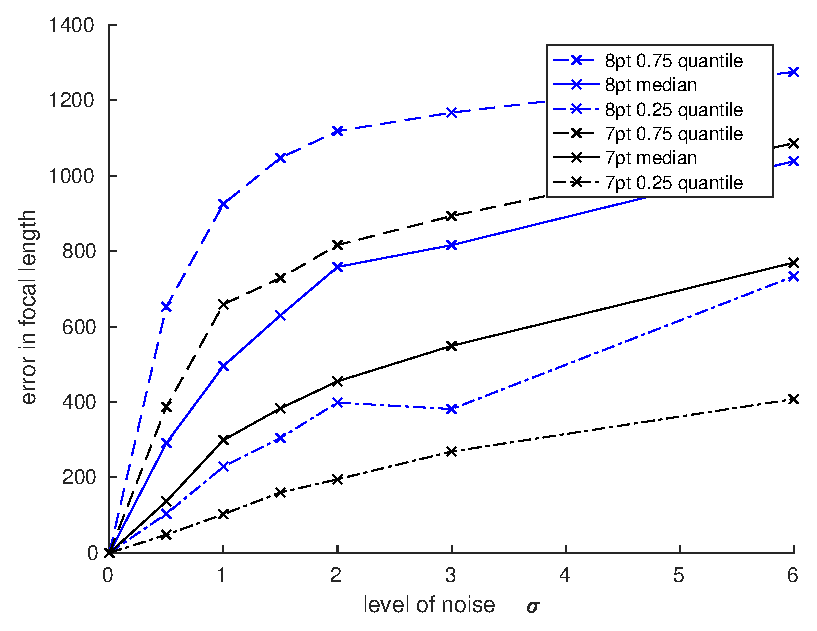
\includegraphics[width=\linewidth]{mean_error_noise.eps}
    \caption[Error in focal length versus level of noise]{A comparison of the 7pt and 8pt algorithms against noise level $\sigma$. The ground truth $f^{true}$ is equal to 1500. 40 correspondences are used.}
    \label{mean_v_noise}
  \end{center}
\end{figure}

Another important trend  is shown in the Fig.~\ref{imaginary_number} is the decrease of number of imaginary estimates with increasing number of correspondences used. We suggest that imaginary focal lengths are due to high level of noise, and appear less often when the noise is averaged over a  big number of correspondences.

\begin{figure}[h!]
  \begin{center}
    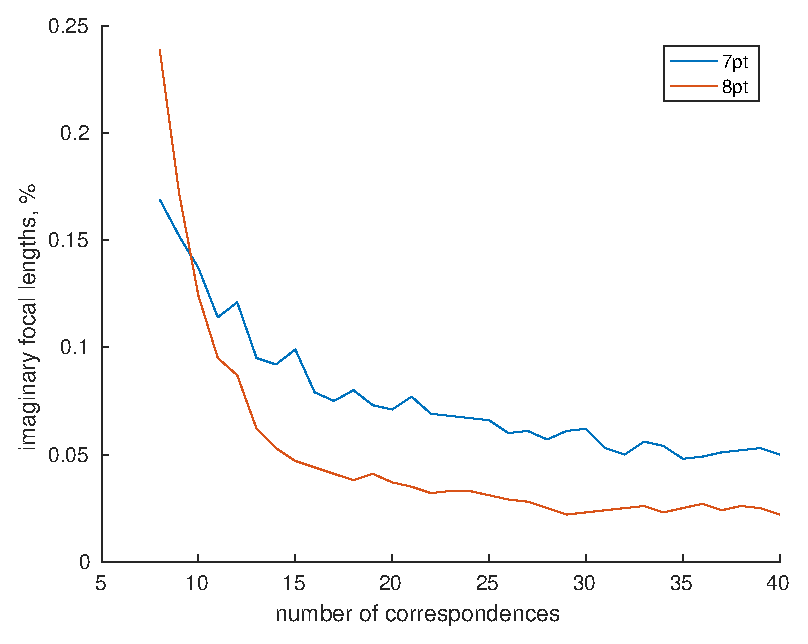
\includegraphics[width=\linewidth]{imaginary_number.eps}
    \caption[Fraction of imaginary focal length estimates versus number of correspondences]{The fraction of imaginary focal length estimates by the 7pt and 8pt algorithms. The noise level $\sigma$ in image measurements is equal to 1. }
    \label{imaginary_number}
  \end{center}
\end{figure}

We conclude that when the estimate of the focal lengths is real we can generally expect it to be quite precise and usable for most practical cases. More correspondences insure good performance, and moderate amounts of noise can be handled well. The 7pt algorithm performs better for most applications, however, interestingly enough, the 8pt algorithm gives less imaginary estimates.

\subsection{Ratio of focal lengths is robust}

We will continue to analyze the 7pt algorithm, as it apparently performs better than the 8pt algorithm on average. The 7pt algorithm also has the theoretical advantage in that it never gives a matrix of rank 3 (remember that a fundamental matrix is always of rank 2).


We  show empirically that the ratio $r={f_2}\slash{f_1}$  computation is more robust than computation of $f_1$ or $f_2$ alone.
To show it we conduct an experiment with  300 different noise samples applied to the same camera geometry. We exclude extreme outliers.

The Fig.~\ref{scatter} shows scattered estimated points in the space $(f_1,f_2)$. If the distribution of estimates in this space doesn't have additional structure, we expect these estimations to lie around the ground truth, perhaps similar to a two-dimensional Gaussian distribution. However,  it can be seen that while the deviation of focal lengths from the ground truth point is relatively big, the points clearly tend to the line $f_2 \slash f_1= 3\slash4$ (given in blue), which is indeed the ground truth for the ratio. Imaginary estimates are also shown in absolute values, which, interestingly, also tend to have the right ratio. We will expand on this in the next section.

We conclude that the computation of the ratio of the focal lengths $r$ by Bougnoux formula is more robust than the the computation of focal lengths themselves by the Bougnoux formula.
We will use this fact later to construct a more robust solver.

\begin{figure}[h!]
  \begin{center}
    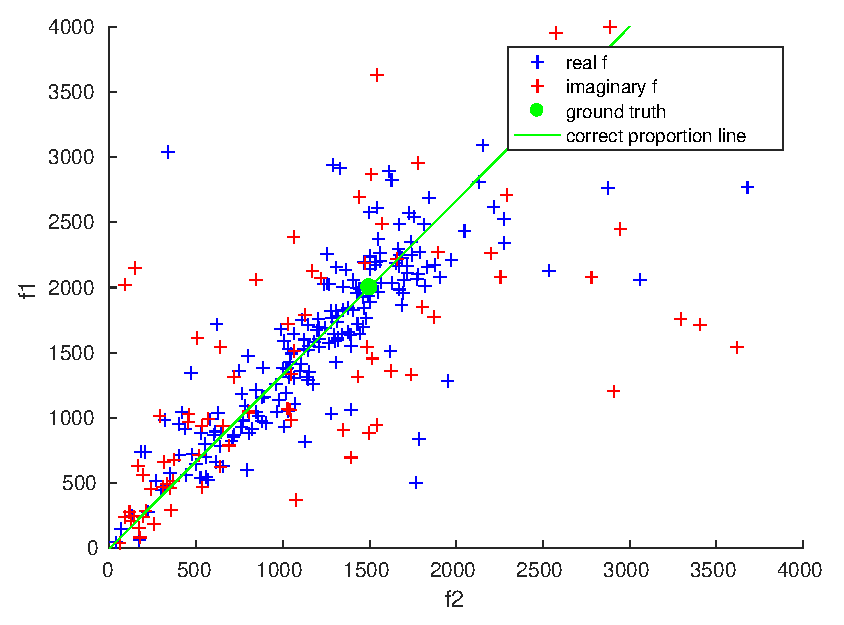
\includegraphics[width=\linewidth]{bougnoux_scatter.eps}
    \caption[Scattered focal length estimates]{The scatter plot of the focal lengths $(f_1, f_2)$ estimates by the 7pt algorithm for one scene. Line through ground truth ratio $r = f_2\slash f_1$ is given for reference. Ground truth point also shown in green. Imaginary estimates are shown in absolute value. The noise level $\sigma$ in image measurements in image measurements is equal to 1. Seven correspondences are used.}
    \label{scatter}
  \end{center}
\end{figure}

\subsection{Imaginary focal lengths}
\label{sec:Imaginary}
We empirically show that the ratio of the focal lengths is robust even when both focal lengths are imaginary.
The probability of getting an imaginary focal length also  isn't connected to distance between optical axes. 

Fig.~\ref{imagist_ratio} shows the experiment. The figure is the histogram of different errors in ratio (measured as $f_2\slash f_1-(f_2/f_1)_{gt}$).  A small number of outliers lies far off the graph.
Clearly, the likelihood that a focal lengths ratio is estimated better is bigger when the focal lengths are real. However, the Fig.~\ref{imagist_ratio} shows that the ratios  computed from imaginary focal lengths also fall reasonably close to the ground truth, in the sense that the mean of their distribution seem to converge to the ground truth ratio.

The distribution of the imaginary focal lengths itself is shown in the Fig.~\ref{imagist}. We see that for bigger values of error, the number of imaginary estimates is roughly equal to the number of real ones, in other words, the likelihood of getting an imaginary focal length estimate is around 50$\%$ when the error in focal length estimate is bigger than twofold. 

 We suggest that there is a hidden variable that is susceptible to noise and makes both focal lengths imaginary when the level of noise is high. It doesn't, however, affect the absolute values of the squares of the focal lengths. The variable seems to be selecting the sign of the square of the focal lengths in a way that the higher the noise is the more probable it is that the sign will be negative. 

 One of our guesses was that the probability of having imaginary estimate can increase when the situation becomes close the degenerate. In the next experiment we assess the degree of degeneracy by the length of shortest transversal between the optical axes. When the length is zero, the optical axes intersect. 

The Fig.~\ref{scatter_imaginary} shows the estimated ratios $r=f_2\slash f_1$. We see that the fraction of imaginary estimates does not depend on the length of shortest transversal. We also see how both ratios computed from real and imaginary estimates tend to the ground truth. We plot the ratios estimated from imaginary values of the focal lengths with negative sign and in red to distinguish it from the ratios estimated from the real values, which are shown in blue.


\begin{figure}[h!]
  \begin{center}
    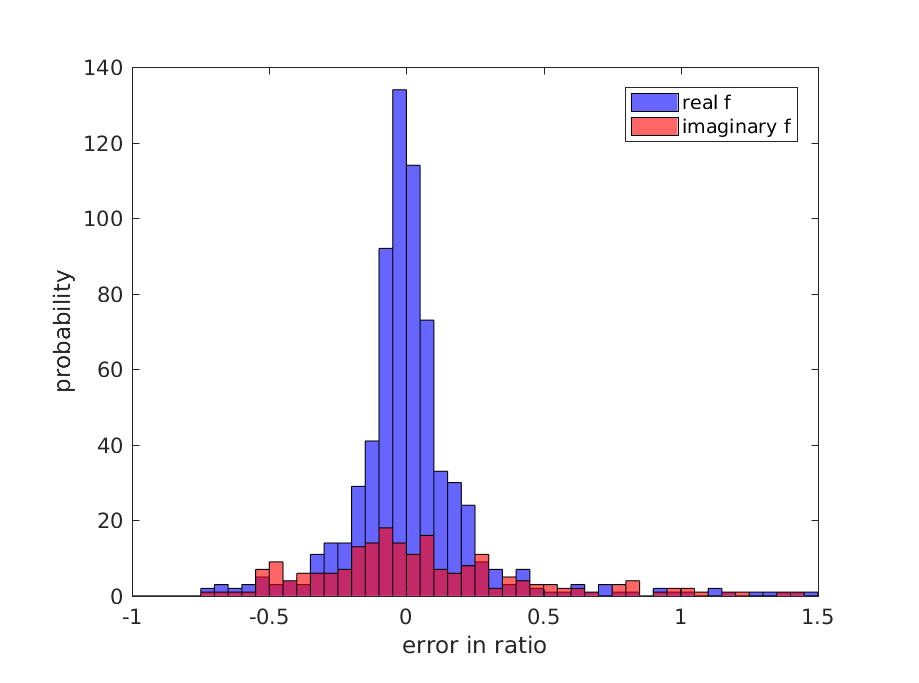
\includegraphics[width=\linewidth]{imaginary_hist_ratio.eps}
    \caption[Histogram of errors in the ratio of the focal length]{The histogram of errors in the ratio of focal length estimations by 7pt algorithm, i.e.\  $f_2 \slash f_1 - f_2^{true} \slash f_1^{true}$ . The cases with at least one imaginary focal length are shown in a separate histogram (orange), the cases where both focal length were real are shown in blue.  Red color is shown where an orange is supersimposed over blue. 40 correspondences are used, and level of noise $\sigma$ is equal to 1. A small number of outliers lies far off the graph.}
    \label{imagist_ratio}
  \end{center}
\end{figure}


\begin{figure}[h!]
  \begin{center}
    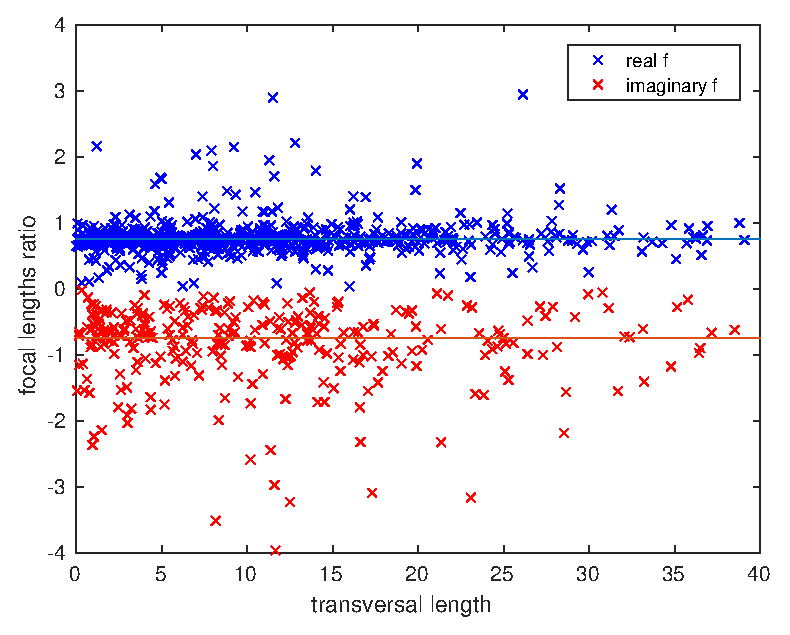
\includegraphics[width=\linewidth]{scatter_imaginary.eps}
    \caption[Scattered focal length ratio estimates]{Scatter plot of focal lengths ratio $r=f_2\slash f_1$ estimates produced by 7pt algorithm. Ratios corresponding to imaginary focal lengths are plotted as negative to distinguish them (they are positive). On $X$ axis is the distance between optical axes.  A small number of outliers lies far off the graph.. 40 correspondences are used. }
    \label{scatter_imaginary}
  \end{center}
\end{figure}

\begin{figure}[h!]
  \begin{center}
    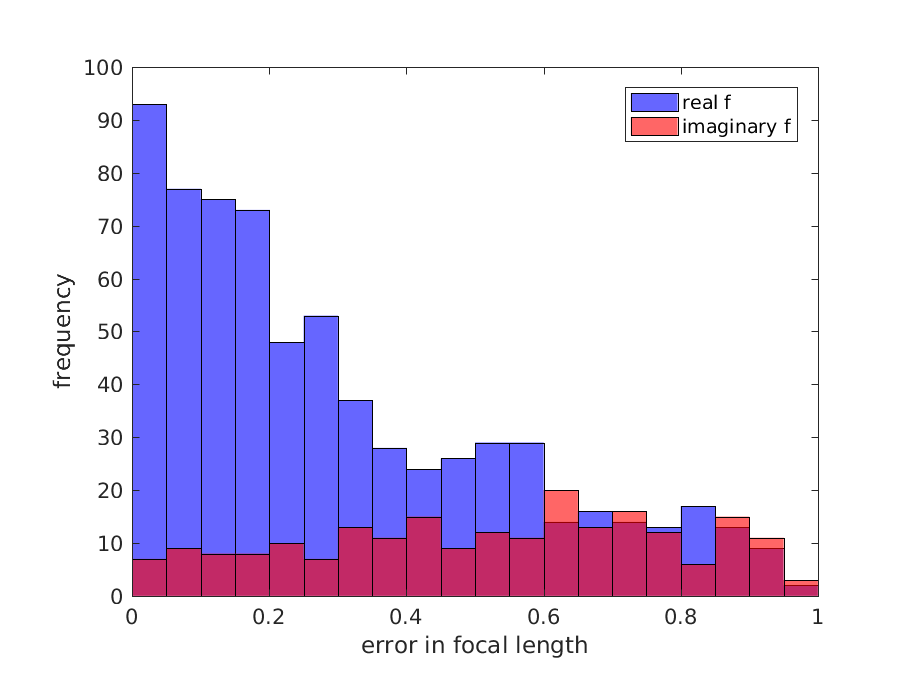
\includegraphics[width=\linewidth]{imaginary_hist.eps}
    \caption[Histogram of errors in the focal length]{The distribution of multiplicative errors (equation \ref{eq:error}) in the focal lengths, produced by 7pt algorithm. Separate distributions are shown for the  case with both real focal lengths (blue) and for the case with at least one imaginary focal length (orange). Red color is shown where the orange is supersimposed over blue. 40 correspondences are used, and level of noise $\sigma$ is equal to 1. }
    \label{imagist}
  \end{center}
\end{figure}


\section{Performance analysis for close to degenerate situations}

In theory, there does not exist a method to recover focal length when the optical axes intersect. With a small amount of noise in the image measurements, however, the configuration no longer is singular. The focal lengths  thus can be computed in almost all practical situations. Nonetheless, we expect pose estimation to deteriorate as the configuration becomes close to singular due to numerical instability. In this section we show the extent of this deterioration.  For the fundamental matrix estimation, we will use the 7pt algorithm, as it apparently performs better than the 8pt algorithm.

\subsection{Intersecting optical axes} 

In this scenario, two non-parallel optical axes are initially in a plane and we lift one camera away from the plane to distance $d$. The optical axes become skew lines. We compare the quality of estimations for different distances $d$ and levels of noise $\sigma$.
In our setup the distance between camera centers is 1 m and the mean distance from the cameras to the scene points is 5 m. 

The Fig.~\ref{interax} shows the distribution of multiplicative errors in the focal length estimates by the 7pt algorithm. The figure shows 4 different levels of noise, and each line represent a distance $d$. We see that for small values of noise, $\sigma \ll 0.1~\text{px}$, the distance between the optical axes significantly affects 7pt algorithm performance.
The performance  deteriorates greatly with decreasing distance between optical axes. For more realistic noise levels, however, the Fig.~\ref{interax} shows that the distance has little impact on the quality of estimation. With 1 pixel noise, the performance is almost the same and axes that are 10 cm or 1 cm apart. A 50 cm transversal configuration, which we assume is not influenced by the degeneration is marginally more suitable for reconstruction. Even for configuration with axes distance zero, the performance is still acceptable (because of the noise in image measurements), with 75\% of estimations being off by a factor of at most 2. 

We suggest this happens because the  noise in image measurements drives the system further away from a degenerate situation. %\TP{delet: The noise effect on camera geometry aprarently has a bias towards moving optical axes further from each other, which reduces the effect of numerical instability.} 


\begin{figure}[h!]
  \begin{center}
    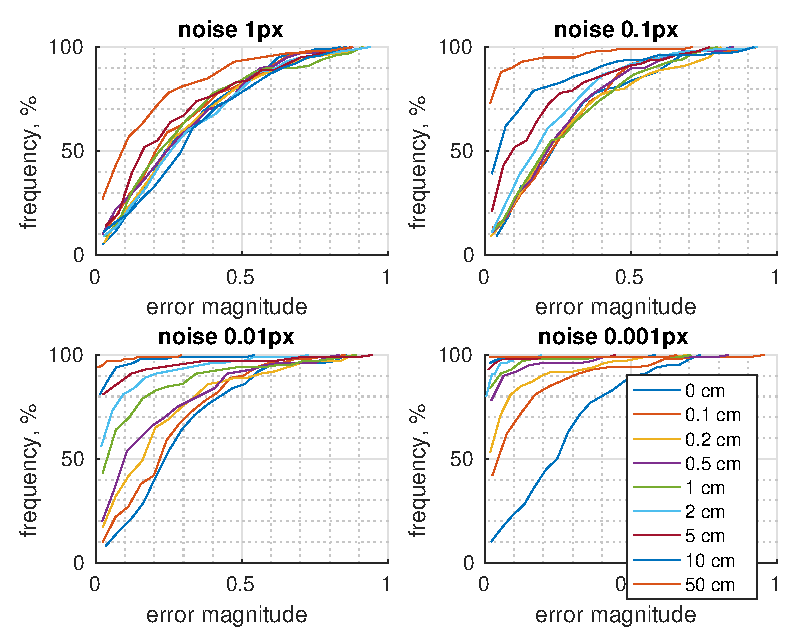
\includegraphics[width=\linewidth]{foc_err_intersecting_axes.eps}
    \caption[Focal length error for intersecting optical axes]{The cumulative distribution of the estimated focal length multiplicative error (equation \ref{eq:error}) for nearly intersecting optical axes. Different lines show different distances between optical axes in centimeters. 7pt algorithm is used}
    \label{interax}
  \end{center}
\end{figure}

\subsection{Parallel optical axes}
An interesting configuration is when the optical axes intersect at a point at infinity, i.e., when they are parallel.

In this scenario, two optical axes are initially parallel and we rotate one axis away from the common plane of the axes by  angle $\alpha$. As we rotate one axis away, it is no longer parallel to the other one. We compare the quality of estimations for different angles $\alpha$ and levels of noise $\sigma$.

Fig.~\ref{parallax} shows the results. We see that the quality of estimation is much worse for  truly parallel axes and small noise in image correspondences does not save the situation. However, the degeneracy almost disappears already when the angle $\alpha$ reaches $0.1^\circ$.


\begin{figure}[h!]
  \begin{center}
    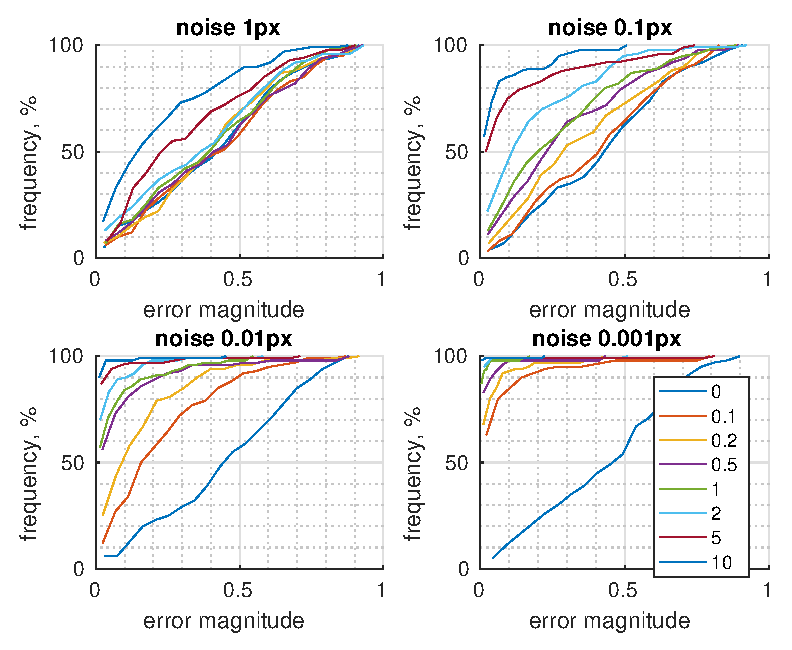
\includegraphics[width=\linewidth]{foc_err_parallel_axes.eps}
    \caption[Focal length error for parallel optical axes]{The cumulative distribution of the estimated focal length multiplicative error (equation \ref{eq:error}) for nearly parallel optical axes. Different lines show different angles between optical axes in degrees. 7pt algorithm is used}
    \label{parallax}
  \end{center}
\end{figure}

\subsection{Conclusions}

We have shown that the 7pt algorithm performs better for most applications. However, interestingly, 8pt algorithm gives less imaginary estimates.

Using more correspondences allows us to make much better results and get imaginary estimates less often. The ratio $r = {f_2}\slash{f_1}$ seems to be more robust than the focal lengths themselves. The ratio is also usable even when the focal lengths are imaginary. 


We confirmed that the imaginary focal lengths are indeed signs of a highly corrupt solution, and the fundamental matrices that decompose into imaginary focal lengths should be discarded.  

Of two types of camera configuration degeneracy, intersecting optical axes do not pose a significant risk for camera reconstruction, especially for real-life noise levels. A configuration with parallel or nearly parallel optical axes, however, is a harder case where more than a half of reconstructions may be off by a factor of two and more.
